\documentclass{article}

\usepackage{graphicx}
\usepackage{placeins}
\usepackage{fancyhdr}
\usepackage{longtable}
\usepackage{lastpage}
\usepackage{rotating}
\usepackage{pdfpages}
\usepackage[hidelinks]{hyperref}
\usepackage{todonotes}

% clear the default headers
\fancyhead{}
\fancyfoot{}

\renewcommand{\headrulewidth}{0pt}
\renewcommand{\footrulewidth}{0pt}

\newcommand{\projName}{APO Chapter Organization Website}
\newcommand{\docName}{Software Design Document}
\newcommand{\docVersion}{Version 1.0}
\newcommand{\docDate}{October 10, 2012}

\newcommand{\specialcell}[2][c]{\begin{tabular}[#1]{@{}c@{}}#2\end{tabular}}

\setlength\LTleft{0pt}
\setlength\LTright{0pt}

\fancypagestyle{plain}{

\headheight=10mm
\fancyhead{\begin{longtable}{@{\extracolsep{\fill}}|l|r|}
\hline
\projName & \docVersion \\ \hline
\docName & \docDate \\ \hline
\end{longtable}}

\fancyfoot[C]{\footnotesize Page \thepage\ of \pageref{LastPage}}}

\pagestyle{plain}

\setcounter{tocdepth}{2}

\title{\projName \\ \vspace{10 mm}
\docName \\ \vspace{10 mm}
Devin Schwab\\
Jon Chan}

\date{\docDate}

\begin{document}
\bibliographystyle{IEEE}

\maketitle

\newpage

\begin{longtable}{|l|l|l|l|}
\hline
{\bf Date} & {\bf Version} & {\bf Description} & {\bf Authors} \\ \hline
10/8/12 & Version 0.5 & Initial Draft & Devin Schwab, Jon Chan \\ \hline
\end{longtable}

\newpage

\tableofcontents
\listoffigures

\newpage

\section{Introduction}

\subsection{Document Overview}
The \projName is a new website designed to replace the existing website.
The current website provides basic administrative features for some of the executive positions.
It also provides some basic features that allow brothers to keep in touch. However, each semester
more features are requested and the current website was not designed with future maintainability
in mind. For this reason this project seeks to make a new website that will provide better
administrative tools and better social tools. The goal is for the website to decrease the amount of effort
needed for administration and to get chapter members more involved in the organization. This document lays out
the design for the new website including the overall architecture, rationale for selected components and
services and the specifications of new components and services which must be created.

\subsection{Document Conventions}
This document references previous documents created for this project as well as documentation
for outside systems this system will interact with. References for the system can be found at the end of the document.
In text citations are listed as numbers in square brackets. For example ``[ 1 ]''. 

\subsection{Definitions and Acronyms}

% Add definition to the table
\begin{tabular}{p{.20\textwidth}p{.80\textwidth}}

\multicolumn{2}{c}{ {\bf Definitions} } \\ \hline
{\bf Brother} & A general member of the chapter that has gone through the pledging process. \\ \hline
{\bf Contract} & The requirements that a member must satisfy to remain in good standing with the chapter \\ \hline
{\bf Exec Member} & A general member of the chapter (brother) that is elected or appointed to run a specific aspect of the chapter. \\ \hline
{\bf Membership Review} & Event at the end of the semester in which the completion of each member's contract is reviewed by the chapter\\ \hline
{\bf Pledge} & A member who has completed the initiation ceremony, but not the induction ceremony. These members do not have the full privilege of a brother\\ \hline
{\bf Rushee} & A person who is interested in joining APO, but is not yet a pledge \\ \hline
{\bf Service Report} & Request for approval of community service hours\\ \hline
{\bf Alumni} & A person who was previously a member, but has since graduated\\ \hline
\end{tabular}

\begin{tabular}{p{.20\textwidth}p{.80\textwidth}}
\multicolumn{2}{c}{ {\bf Acronyms} } \\ \hline
GAE & Google App Engine \\ \hline
SSL & Secure Socket Layer \\ \hline
\end{tabular}

\section{Website Architecture}

\subsection{General Web Architecture}

The basic architecture follows a design pattern for the website.

\FloatBarrier
\begin{figure}[h!]
\missingfigure{General Web Architecture}
\caption{General Web Architecture}
\label{fig:generalWebArchitecture}
\end{figure}
\FloatBarrier

Multiple users connect to a webserver running our software and database via the Internet.
Setting up a webserver also requires setting up a Domain Name System (DNS) server and registering a domain
name.

The following subsections detail design decisions for each aspect of this general architecture.

\subsection{Webserver - Google App Engine}

As shown in figure \ref{fig:generalWebArchitecture} part of the architecture is the webserver which will run the actual application. There are two main options
for the webserver: buy a computer and configure it to be a webserver or use a hosting service. In the vision and scope document for this project
one of the assumptions was that the website will be hosted for free and that the website will be provided with a free
domain name. \cite{schwab_apo_2012} This rules out the buy and configure a webserver option. So it is necessary to select a free hosting service.

There are a multitude of free hosting services on the web, but the services vary in quality and not all packages
come with a free domain name. The free services are often limited in the amount of bandwidth and storage they can use.
Out of the surveyed hosting services with free packages Amazon EC2 offered the most amount of free bandwidth and storage. \cite{amazon_amazon_2012} \cite{heroku_heroku_2012} \cite{google_quotas_2012} However, using Amazon EC2 would require setup and configuration of a webserver and database server. In addition Amazon EC2's free tier is only free for the first year. After which the user must pay for all services.

On the other hand Google App Engine (GAE) has a free tier that does not expire. The amount of resources provided for free are not as high as Amazon's free tier, but the service will remain free for the foreseeable future.  \cite{google_quotas_2012} 

In addition GAE provides a free hostname by giving the application a subdomain of the appspot.com domain. This means
that a domain name will not need to be purchased and no DNS server will need to be purchased and configured.
An additional benefit of GAE is that the free domain also comes with a free Secure Socket Layer (SSL) Certificate. An SSL 
certificate will be needed to provide secure login pages and to encrypt and authenticate sensitive information.

\subsection{Database - Google's Bigtable Datastore}

Another part of the architecture shown in figure \ref{fig:generalWebArchitecture} is the database. Traditional web
applications use a Structured Query Language (SQL) based database such as MySQL. However, by choosing GAE as the hosting service the website
is restricted to using Google's Bigtable Datastore.

The advantage of this constraint is that the website's data is very unlikely to be lost due to Google's large number
of resources. In addition defining the schema for the Bigtable datastore is much easier than in a traditional SQL database.
This is because Bigtable is what is known as a ``NoSQL'' database. \cite{google_how_2012} ``NoSQL'' essentially means that the database does not have a traditional SQL schema. This means that instead of using tables like a traditional
SQL database Bigtable uses one ``big table'' that store what are known as ``Entities''. Entities are instances of a ``Model''. Models define the datatypes stored in an Entity as well as the requirements for each field. Models are defined in the code meaning that
the schema can easily be modified. Additionally the schema is automatically version controlled because it is defined in the
code that is already under version control. Models are also object oriented meaning that a base model can be defined and
generalized to more specific models. All of these properties make the Google's Bigtable more flexible than a traditional
database.

The one big disadvantage of Bigtable is that being a datastore type database there is no such thing as a JOIN operation. 
Instead any JOIN-like operation must be implemented by the developers.

\subsection{Application Language - Python}

Another constraint imposed by the choice of GAE is the language the website can be written in. GAE applications can
be written in Python, Java, or any other JVM compatible language. \cite{google_google_2012}

Out of the possible languages Python will be used. Python is cross platform meaning that all developers can
work on the code regardless of what their operating environment is. Additionally the Python language has been supported
longer by GAE meaning that the documentation and support is more mature. This will allow developers to worry less about
unsupported features of the language on the hosting platform and more about the actual functionality of the code.

\subsection{Application Framework - Flask}

GAE does not require that a web framework is used. However, if a Python based web framework is not used then a lot of
the development time will be spent implementing the underlying components of a Python Web Server Gateway Interface (WSGI) server application. \cite{wsgi.org_what_2012} Dozens of WSGI server frameworks have been written, such as Flask and Django. \cite{_flask_2010} \cite{_django_2012} It makes no sense to waste development time working on code that already exists. For this reason a Python based web development framework has been chosen.

Of the two mentioned frameworks, Django and Flask, Flask has been chosen as the framework the website will use. Of
the two Flask makes less design decisions for you. For instance Django assumes that the projects built on top of it will
use Django's database interface. However, that interface will not work with GAE's Bigtable datastore. It is possible to configure Django to use a different database, but it is difficult. Flask on the other hand is considered a ``microframework''.
According to Flask's website this means that while Flask gives the projects built on it the basic code such as the WSGI 
interface, Flask tries not to make higher level design decisions. Additionally Flask has many plugins available on
their website. \cite{extensions_flask_2012}

\subsection{Photo Storage - Photobucket}

Something that is not part of the general web architecture depicted in figure \ref{fig:generalWebArchitecture} are outside
web services that this website would be communicating with. This website will need to communicate with an outside site to satisfy requirements REQ-32 through REQ-36 and their respective subrequirements. \cite{schwab_apo_srs_2012}

Those requirements could be satisfied by storing the photos on the GAE service. However, the free storage space is limited
on GAE. If users want to upload high resolution photographs the free storage will quickly run out. To mitigate this problem
the website will communicate with one of the many photo sites on the web. For this design Photobucket has been chosen. \cite{_photobucket_2012}

Photobucket is the photo site currently used by the chapter. However, in the user survey included in appendix A of 
the software requirements document many responses included complaints about how difficult it was to use.\cite{schwab_apo_srs_2012}  Choosing Photobucket as the outside photo service the website will have access to the existing photos on Photobucket.

Photobucket's API does have limits on the amount of operations an application can perform before being charged. \cite{photobucket_method_2010} However, the limits are well beyond the expected traffic for this website.

Photobucket's API is authenticated using OAuth meaning that a developer account will need to be created and a key for the
website will need to be generated. \cite{photobucket_faq_2010}

\subsection{Member Avatars - Gravatar}

Another outside service this website will be using is Gravatar. \cite{_gravatar} Gravatar allows users to upload a photo which can be used across multiple websites as an avatar. To use the avatar a user has on their account the only thing that is needed
is the email address associated with the email on the user's Gravatar account. 

To use the Gravatar account the website only needs to store the email associated with the Gravatar account. The website
can then use the algorithm documented on the Gravatar website to generate the URL for the avatar.

\subsection{APO Chapter Website Architecture}

Taking into account all of the previous design decisions the architecture in figure \ref{fig:generalWebArchitecture}
becomes the architecture depicted in figure \ref{fig:finalWebArchitecture}.

\FloatBarrier
\begin{figure}[h!]

\missingfigure{Website Architecture}
\caption{Website Architecture}
\label{fig:finalWebArchitecture}
\end{figure}
\FloatBarrier

\section{Application Architecture}

\subsection{Main Components}

There are four main types of components that the application is made from

\begin{enumerate}
\item Views
\item Templates
\item Forms
\item Models
\end{enumerate}

Each of these components is described in section \ref{sec:Views} through section \ref{sec:Models}.

\subsubsection{Views}
\label{sec:Views}

A view in Flask is a function or class that handles a web request. The view has one or more URL's routed to it through Flask's URL system. The general program flow for a View is shown in figure \ref{fig:ViewProgramFlow}.

\FloatBarrier
\begin{figure}[h!]
\missingfigure{General View Procedure Flow}
\caption{General View Procedure}
\label{fig:ViewProgramFlow}
\end{figure}
\FloatBarrier

The View starts off by taking in the user request object provided by Flask. The request object contains all of the information
about the web request including the type (e.g. POST or GET). The View takes the information in the request and runs 
any internal procedures needed to process the data. These internal procedures may include things like querying the datastore. Finally the View renders the associated template. While rendering the template the View will pass in any parameters that change from render to render. Finally the View returns the rendered template to Flask which passes it back
as an HTML/javascript page to the user who initiated the request.

\subsubsection{Templates}
\label{sec:Templates}

There are many HTML templating languages for Python. Flask defaults to using Jinja2. \cite{_jinja2_2008} Jinja2 allows basic logic
in the templates and can accept Python objects to be displayed in the rendered page.

Jinja2 also supports inheritance. \cite{ronacher_jinja2_2008} A template can contain what are known as ``blocks''. Blocks can be overridden by 
templates that inherit from the main template where the block was defined. This allows a site to have a hierarchical template
definition. For instance a website can have a main template which includes the static parts of a page that never change
and each individual page can extend the page and add their own content.

\subsubsection{Forms}
\label{sec:Forms}

To support server side form validation the WTForms package is being used with the Flask-WTF extension. \cite{wtforms_team_wtforms_2010} \cite{_flaskWTF} Forms are defined via subclasses of the main form class. The subclassed forms specify the specific fields
as well as their validation criteria. A View can use an instance of the form to render the HTML form elements on a page
and to validate that the received form data meets the criteria specified in the class.

\subsubsection{Models}
\label{sec:Models}

Google's Bigtable requires the definition of Models instead of a traditional schema. Models are inheritable. The website models are subclasses of one of the three following classes: PolyModel, Model, Expando. PolyModel derived classes support inheritance. Model derived classes are the standard model type. Expando derived classes support having additional fields stored with an entity of the model even when that additional data was not specified in the original model.

In this document's diagrams Models are shown as classes (because they are implemented as classes). References are shown by denoting a member variable's type as the type of a model defined in this document.

\subsection{Packages}

There are four main packages. Each package contains the definitions of one of the component types specified in section \ref{sec:Views} through section \ref{sec:Models}. The package structure is show in figure \ref{fig:PackageStructure}.

\FloatBarrier
\begin{figure}[h1]
\centering
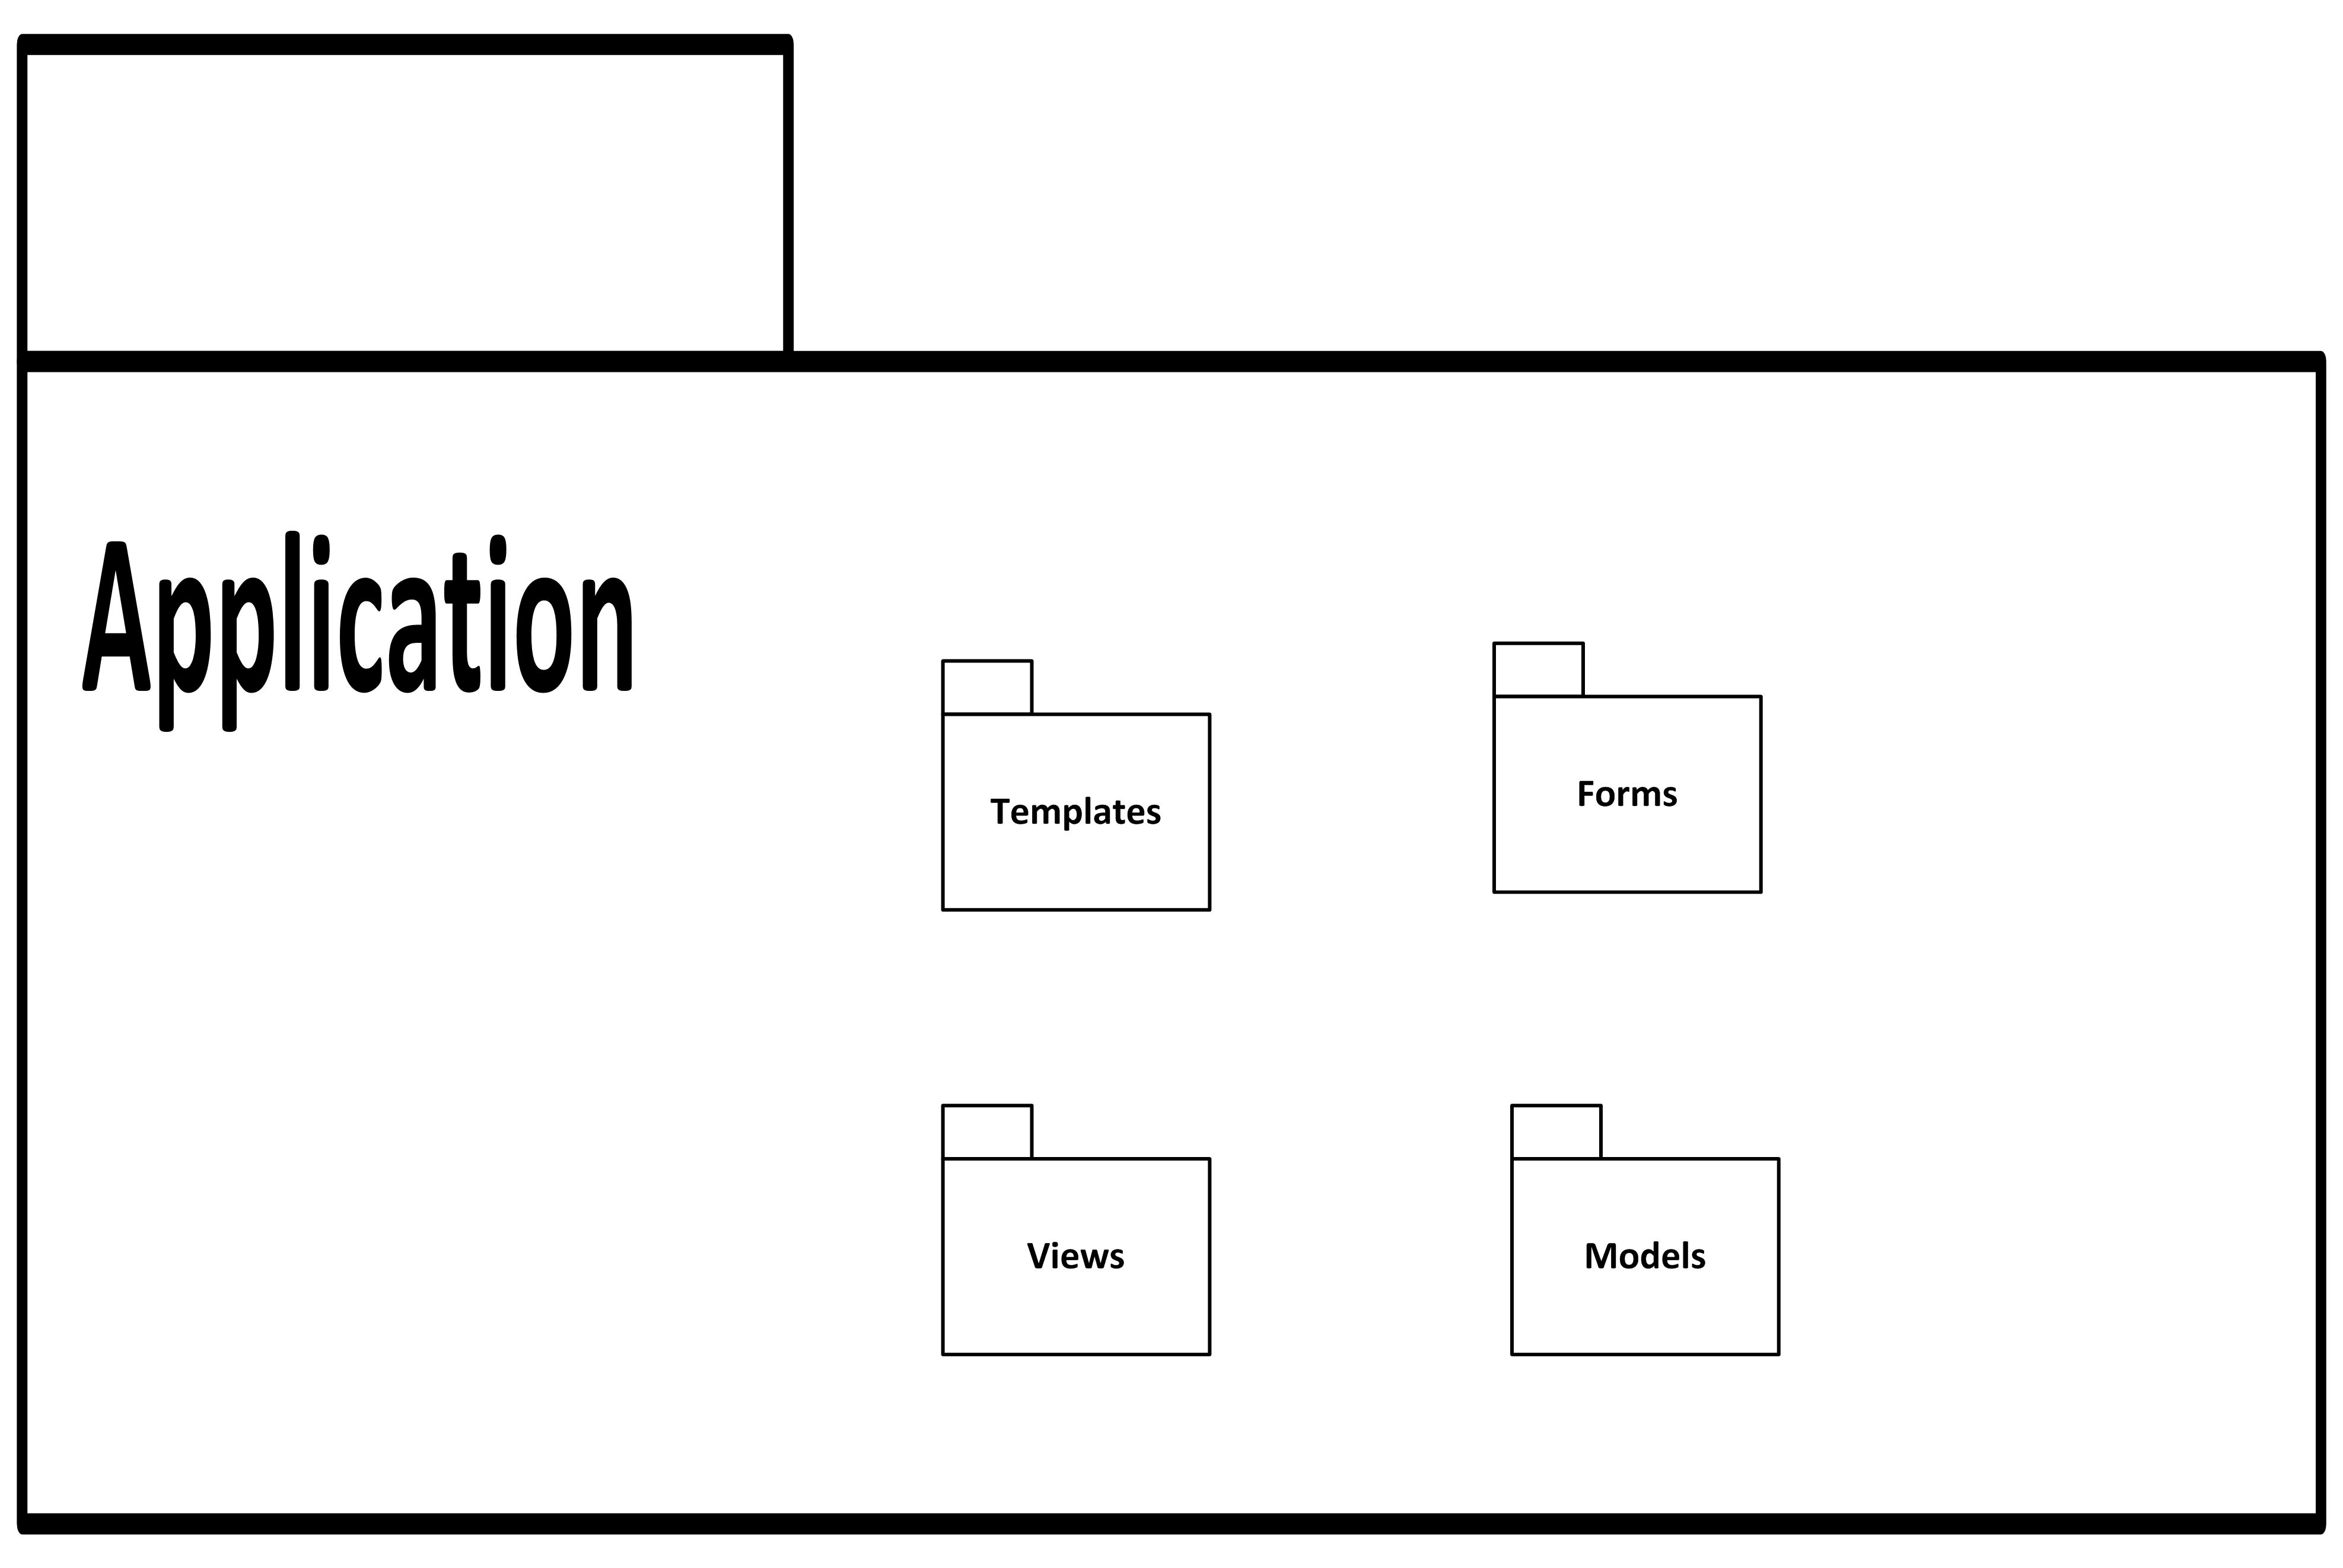
\includegraphics[scale=.75]{img/applicationStructure}
\caption{Package Structure}
\label{fig:PackageStructure}
\end{figure}
\FloatBarrier

\subsection{User Login}

\subsubsection{Flask Login Overview}

In general Flask does not provide anything but the WSGI interface for an application. However, Flask's website links to many
extensions to Flask. User Login is such a common task that an extension to Flask known as Flask-Login exists.

\subsection{User Roles}

\subsubsection{Flask Principal Overview}

\subsection{Photo Classes}

\subsubsection{Photo Class}

\subsubsection{Album Class}

\subsection{Oauth}

Photobucket's API requires the use of Oauth. Oauth is a protocol that allows users of different websites to delegate access
to parts of their account without giving away the account password. Oauth's protocol is specified in RFC 5849, however, because Oauth is so popular multiple libraries implementing the protocol are available for Python. \cite{eranhueniverse_oauth} The library recommended by the maintainers of the Oauth protocol is ``python-oauth2 library'' which can be found on Github. \cite{oauth_code} \cite{simplego_python-oauth2_2011}

\newpage

\bibliography{designBib}

\end{document}